% Лабораторная работа по криптографии № 2
% Дуников Константин Артёмович 

% Тип документа: статья, на бумаге А4
\documentclass[a4paper]{article}

% Подключение сторонних tex файлов 
\usepackage{import}


% Основные данные - ВУЗ, факультет, город...
\import{./../../stuff/tex}{config.tex}
% Небольшой набор инструментов
\import{./../../stuff/tex}{tools.tex}

% Подключение необходимых зависимостей
\import{./../../stuff/tex/settings}{packages.tex}
% Настройка подключенных пакетов
\import{./../../stuff/tex/settings}{preferences.tex}


% Шаблон титульной страницы 
\import{./../../stuff/tex/templates}{title.tex}
% Упрощенный блок "выполнил"
\import{./../../stuff/tex/templates}{sign2.tex}
% Макрос для содержания
\import{./../../stuff/tex/templates}{toc.tex}

% Определяем название документа
\title{
  ОТЧЕТ \\
  О ПРАКТИЧЕСКОЙ РАБОТЕ №2 \\
  по дисциплине <<Криптографические методы защиты информации>> \\
  Современные симметричные шифры
}
% Указываем преподавателя
\renewcommand{\teachername}{
    Заведующий кафедрой информационной безопасности киберфизических систем \\
    канд. техн. наук, доцент \\
    О.О. Евсютин
}

\setminted{fontsize=\footnotesize,baselinestretch=1}

% Путь до внешних изображений
\graphicspath{ {./figures/}}
% Нумеруем все формулы
\mathtoolsset{showonlyrefs=false}

\usepackage{caption}
\newenvironment{code}{\captionsetup{type=listing}}{}

% Основной текст работы
\begin{document}
  \templatedtitlepage
  
  \toc

  \section{Здание на практическую работу}
  В ходе данной работы необходимо:
  \begin{enumerate}
    \item Написать программную реализацию шифра <<Магма>>, описанного в стан-дарте ГОСТ Р 34.12-2015
    \item Подготовить отчёт о выполненной работе
  \end{enumerate}

  Программная реализация должна иметь следующий функционал:
  \begin{enumerate}
    \item Принимать на вход текст, подлежащий зашифрованию/расшифрованию
    \item Принимать на вход секретный ключ
    \item Осущевстлять зашифрование или расшифрование по выбору пользователя
  \end{enumerate}

  Отчёт о выполнении данной практической работы должен включать в себя:
  \begin{enumerate}
    \item Описание задания на практическую работу
    \item Теоретическую информацию о реализуемом шифре
    \item Описание особенностей программной реализации
    \item Вывод о проделанной работе
  \end{enumerate}

  \newpage
  \section{Теоретическое вступление}

  Магма - блочный симметричный шифр, описанный в стандарте ГОСТ Р 34.12-2015.
  Секретный ключ для данного шифра должен иметь длину в 256 бита (8 бит), а размер
  блока (единицы шифрования) - 64 бит (8 байт). Шифр основан на сети Фейстеля,
  является итерационным и использует для работы 32 раунда.

  \subsection{Сеть Фейстеля}

  Сеть Фейстеля - набор ячеек Фейстеля, последовательно соединенных между собой.
  Каждая ячейка представляет собой элемент, принимающий на вход данные и ключ.
  Она делит исходные данные на две равные части - $L$ и $R$. На выход
  каждый ячейка возвращает данные, состоящие из неизмененной части
  $R$ и части $P$, полученной путем побитового сложения $L$ и зашифрованной
  при помощи некой внешней функции шифрования и ключа.

  \begin{figure}[H]
    \centering
    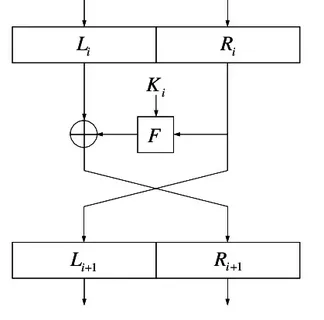
\includegraphics[width=0.5\textwidth]{16_1}
    \caption{Структура ячейки Фейстеля}
  \end{figure}

  Для <<Магмы>> функция шифрования внутри ячейки Фейстеля является
  комплексной и включает в себя использование циклического побитового сдвига
  и замены по специальной таблице.

  \section{Программная реализация}

  Код написан на C++ без использования сторонних бибилиотек.

  Матрица, используемая для замен:
  \begin{minted}{c++}
static constexpr std::array<std::array<ui8, 16>, 8> pi = {
    {12, 4, 6, 2,10, 5,11, 9,14, 8,13, 7, 0, 3,15, 1},
    { 6, 8, 2, 3, 9,10, 5,12, 1,14, 4, 7,11,13, 0,15},
    {11, 3, 5, 8, 2,15,10,13,14, 1, 7, 4,12, 9, 6, 0},
    {12, 8, 2, 1,13, 4,15, 6, 7, 0,10, 5, 3,14, 9,11},
    { 7,15, 5,10, 8, 1, 6,13, 0, 9, 3,14,11, 4, 2,12},
    { 5,13,15, 6, 9, 2,12,10,11, 7, 8, 1, 4, 3,14, 0},
    { 8,14, 2, 5, 6, 9, 1,12,15, 4,11, 0,13,10, 3, 7},
    { 1, 7,14,13, 0, 5, 8, 3, 4,15,10, 6, 9,12,11, 2}
};
  \end{minted}

  Операция замены байт блока шифрования на значения из матрицы выше:
  \begin{minted}{c++}
auto t(ui32 a) -> ui32 {
    ui32 result = 0x00000000;

    for (std::size_t i{0}; i < 8; i++) {
        ui8 ai = (ui8)((a >> (i * 4)) & 0x0000000f);
        ui8 ti = pi[i][ai];

        result = result | ((ui32)(ti) << (i * 4));
    }

    return result;
}
  \end{minted}

  Операция шифрования, применяемая внутри ячейки Фейстеля (замена из предыдущего блока и циклическое смещение на 11 бит):
  \begin{minted}{c++}
auto g(ui32 a, ui32 k) -> ui32 {
    static const ui64 SUM_MOD = std::pow(2, 32);
    ui32 tAkSum = t(((ui64)(a) + (ui64)(k)) % SUM_MOD);
    return (tAkSum << 11) | (tAkSum >> (32 - 11));
}
  \end{minted}

  Непосредственная реализация ячейки Фейстеля:
  \begin{minted}{c++}
auto G(ui32 a1, ui32 a0, ui32 k) -> std::pair<ui32, ui32> {
    return std::make_pair(a0, g(a0, k) ^ a1);
}
  \end{minted}

  \newpage
  И функция зашифрования на основе сети Фейстеля:
  \begin{minted}{c++}
ui64 encrypt(ui64 a, const std::array<ui32, 32>& keys) {
    ui32 a1 = static_cast<ui32>(a >> 32);
    ui32 a0 = static_cast<ui32>(a & 0x00000000ffffffff);

    for (std::size_t i{0}; i < 31; i++) {
        auto temp = G(a1, a0, keys[i]);
        a1 = temp.first; a0 = temp.second;
    }

    return G64(a1, a0, keys[31]);
}
  \end{minted}

  Программа принимает на вход строку, дополняет ее при помощи
  повторе-ния до размера 32 символов и на ее основе генериурет секретный ключ -
  7 раз подряд использует полученную строку, а затем - ее инвертированную версию.

  \subsection{Демонстрация работы программы}

  \begin{figure}[H]
    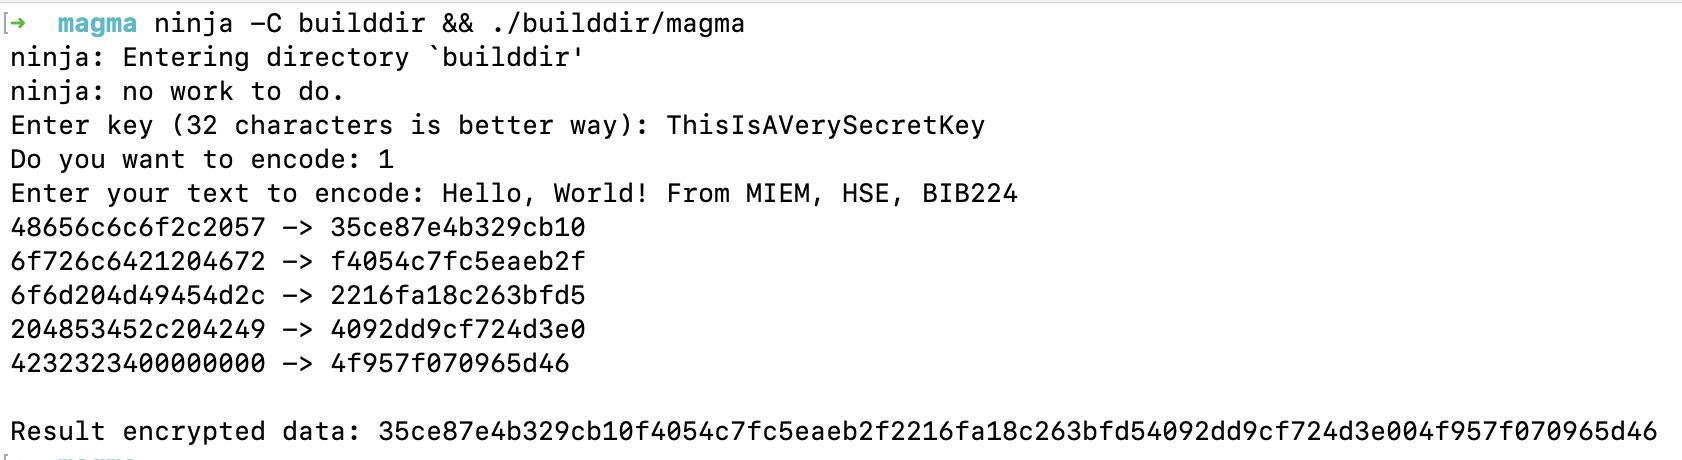
\includegraphics[width=\textwidth]{16_2}
    \caption{Пример зашифрования}
  \end{figure}

  \begin{figure}[H]
    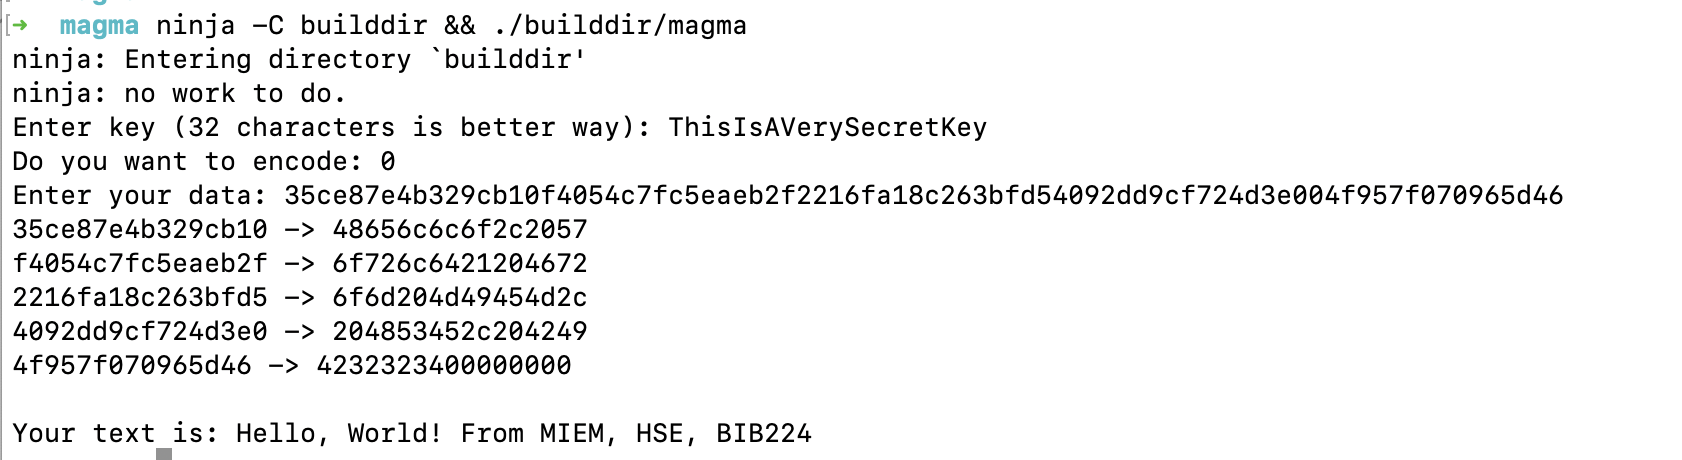
\includegraphics[width=\textwidth]{16_3}
    \caption{Пример расшифрования}
  \end{figure}

  \section{Вывод}

  В ходе данной практической работы была реализована программная реализация
  шифра Магма.

  \end{document}
